\documentclass{setupFiles/final_exam_sust}

%%%%%%%%%%%%%%%%%%%%%%%%%%%%%%%%%%%%%%%%%%%%%%%%%%%%%%%%%%%
%%%%% About prining the solution
\printanswers

%%%%%%%%%%%%%%%%%%%%%%%%%%%%%%%%%%%%%%%%%%%%%%%%%%%%%%%%%%%%%%%%%%%%%%%%%%%%%%%%%%%%%%%
%%%%%%%%%%%%%%%%%%%%%%%%%%%%%%%%%%%%%%%%%%%%%%%%%%%%%%%%%%%%%%%%%%%%%%%%%%%%%%%%%%%%%%%
%%%%% Define all exam variables (Adapt this part for you)

\newcommand{\institutionName}{Shahjalal University of Science and Technology}
\newcommand{\institutionNameShort}{SUST}
\newcommand{\deptName}{Department of Physics}
\newcommand{\deptNameShort}{PHY}


\newcommand{\examName}{1\textsuperscript{st} Year 1\textsuperscript{st} Semester Final Examination,~2022}
\newcommand{\courseCode}{PHY~07131121}
\newcommand{\courseTitle}{Quantum Electronics}
\newcommand{\SessionExaminee}{2020-2021}
\newcommand{\totalMarks}{60}
\newcommand{\totalCredits}{3.0}
\newcommand{\examDuration}{3~Hours}
\newcommand{\examDate}{October~09,~2025~--~14:30} % Exam date or the questing writing date
\newcommand{\specialInstruction}{Answer \textbf{all} the questions.}



\newcommand{\teacherName}{Md Rasedujjaman}
\newcommand{\teacherUniqueID}{N07R28S33}

%%%%%%%%%%%%%%%%%%%%%%%%%%%%%%%%%%%%%%%%%%%%%%%%%%%%%%%%%%%%%%%%%%%%%%%%%%%%%%%%%%%%%%%
%%%%%%%%%%%%%%%%%%%%%%%%%%%%%%%%%%%%%%%%%%%%%%%%%%%%%%%%%%%%%%%%%%%%%%%%%%%%%%%%%%%%%%%
\begin{document}

%%%%%%%%%%%%%%%%%%%%%%%%%%%% The Header of the question %%%%%%%%%%%%%%%%%%%%%%%%%%%%%%%

%%% Title 
%%% Adapat the content accordingly
\begin{center}
	\textbf{\Large{\institutionName{}}}\\[2pt]
	\textbf{\large{\deptName{}}}\\[2pt]
	\textbf{\examName{}}\\[2pt]
	\textbf{Course~Code:~\courseCode{}} \hspace{10mm} \textbf{Session:}~\SessionExaminee\\[2pt]
	\textbf{Course~Title:}~\courseTitle{}\\
	
	
	
\end{center}

%% The Marks, Credits and Times
\vspace{1mm}
\noindent
\makebox[\textwidth]{%
  \textbf{Total~Marks:~\totalMarks{}}%
  \hfill%
  \textbf{Credits:~\totalCredits{}}%
  \hfill%
  \textbf{Total~Time:~\examDuration{}}%
}

%% The horizontal ruller
\vspace{-2.0mm}
\noindent\rule{\textwidth}{2pt}

%% The instruction
\begin{center}
\vspace{-2.0mm}
\textit{[\specialInstruction{}~The figure in the right margin indicate full marks.]}
\end{center}
\vspace{2mm}

%%%%%%%%%%%%%%%%%%%%%%%%%%%%%%%%%%%%%%%%%%%%%%%%%%%%%%%%%%%%%%%%%%%%%%%%
\begin{questions}
	

%%%%%%%%%%%%%%%%%%%%%%%%%%%%%%%%%%%%%%%%%%%%%%%%%%%%%%%%%%%%%%%%%%%%%%%%%%%%%%%%%%%%%%%%%%%%%%%%%%%%%
%%%%%%%%%%%%%%%PART-A(Question#01- Frequency Response of Amplifier //%%%%%%%%%%%%%%%%%%%%%%%%%%
%%%%%%%%%%%%%%%%%%%%%%%%%%%%%%%%%%%%%%%%%%%%%%%%%%%%%%%%%%%%%%%%%%%%%%%%%%%%%%%%%%%%%%%%%%%%%%%%%%%%%	
\question 
\begin{parts}
%%%%%%%%%%%%%%%%%%%%%%%%%%%%%%%%%%%%%%%%%%%%%%%%%%%%%%%%%%%%%%%%%%%%%%%%%%%%%%%%%% 
\part[2] \color{red}If you want to put two or more figures side by side then you can use the latex minipage environment.\color{black} What is super Node? What is the difference between Super Mesh \& Mesh?

\begin{solution}

\end{solution}	
%%%%%%%%%%%%%%%%%%%%%%%%%%%%%%%%%%%%%%%%%%%%%%%%%%%%%%%%%%%%%%%%%%%%%%%%%%%%%%%%%%	
\part[4]Using nodal analysis, determine the potential across the $4~\unit{\Omega}$ resistor in Fig.~\ref{fig:ckt-nodal-analysis} 

\begin{figure}[H]
\centering
%%%%%%%%%%%%%%%%%%%%%%%%%%%%%%%%%%%%%%%%%%%%%%%%%%%%%%%%%%%%%%%%%%%
% First figure
\begin{minipage}[t]{0.48\textwidth}
\centering
\scalebox{0.7}{
\begin{tikzpicture}
% Paths, nodes and wires:
	\draw (4, 4) to[american resistor, l_={$2~\Omega$}, label distance=0.02cm] (7, 4);
	\draw (7, 4) to[american resistor, l_={$2~\Omega$}, label distance=0.02cm] (10, 4);
	\draw (10, 4) to[american resistor, l={$4~\Omega$}, label distance=0.02cm] (10, 1);
	\draw (4, 4) to[american resistor, l={$2~\Omega$}, label distance=0.02cm] (4, 1);
	
	
	
	\draw (4, 4) to[american resistor, l={$5~\Omega$}, label distance=0.02cm] (7, 6);
	\draw (7, 6) to[american resistor, l={$5~\Omega$}, label distance=0.02cm] (10, 4);
	\draw (7, 1) to[american current source, l_={$3~A$}, label distance=0.02cm] (7, 4);
	\draw (4, 1) -- (10, 1);
	\draw node[ground] at (7, 1) {};
	\draw node[ground] at (7, 1) {};
	\draw node[ground] at (7, 1) {};
	\draw node[ground] at (7, 1) {};
\end{tikzpicture}
}
\caption{}
\label{fig:ckt-nodal-analysis}
\end{minipage}
%%%%%%%%%%%%%%%%%%%%%%%%%%%%%%%%%%%%%%%%%%%%%%%%%%%%%%%%%%%%%%%%%%%
\hfill
%%%%%%%%%%%%%%%%%%%%%%%%%%%%%%%%%%%%%%%%%%%%%%%%%%%%%%%%%%%%%%%%%%%
% Second figure
\begin{minipage}[t]{0.48\textwidth}
\centering
\scalebox{0.7}{
\begin{tikzpicture}

% Paths, nodes, and wires:
	\draw (5, 7) to[american resistor, l={$2~\Omega$}, label distance=0.02cm] (5, 4);
	\draw (5, 4) to[american resistor, l={$4~\Omega$}, label distance=0.02cm] (5, 1);
	\draw (8, 7) to[american resistor, l={$8~\Omega$}, label distance=0.02cm] (8, 4);
	\draw (8, 4) to[american controlled voltage source, l={$2~v_o$}, label distance=0.02cm] (8, 1);
	\draw (5, 4) to[american current source, l={$3~A$}, label distance=0.02cm] (8, 4);
	\draw (3, 7) to[american voltage source, l_={$12~V$}, label distance=0.02cm] (3, 1);
	\draw (3, 1) -- (8, 1);
	\draw (3, 7) -- (8, 7);


    \node at (4.5, 5.5) [align=center] {\textbf{+} \\[0.25cm] $v_o$ \\[0.25cm] \textbf{-}}; % Increased spacing above and below V_2


	% Loop current labels:
	\node at (4.0, 4.1) {$i_1$}; % Left loop
	\node at (6.7, 5.6) {$i_2$}; % Middle loop
	\node at (6.7, 2.6) {$i_3$}; % Right loop

	% Loop current direction arrows:
	\draw[->] (3.8, 4.5) arc[start angle=120, end angle=-150, radius=0.5]; % i1 loop arrow
	\draw[->] (6.5, 6) arc[start angle=120, end angle=-150, radius=0.5]; % i2 loop arrow
	\draw[->] (6.5, 3) arc[start angle=120, end angle=-150, radius=0.5]; % i3 loop arrow
\end{tikzpicture}
}



\caption{}
\label{fig:ckt-mesh-analysis}
\end{minipage}
%%%%%%%%%%%%%%%%%%%%%%%%%%%%%%%%%%%%%%%%%%%%%%%%%%%%%%%%%%%%%%%%%%%

\end{figure}

\begin{solution}

\end{solution}
%%%%%%%%%%%%%%%%%%%%%%%%%%%%%%%%%%%%%%%%%%%%%%%%%%%%%%%%%%%%%%%%%%%%%%%%%%%%%%%%%%%%%	
\part[4]Use mess analysis to find currents and voltage $v_o$ in the circuit of Fig.~\ref{fig:ckt-mesh-analysis}
	
\begin{solution}

\end{solution}	
%%%%%%%%%%%%%%%%%%%%%%%%%%%%%%%%%%%%%%%%%%%%%%%%%%%%%%%%%%%%%%%%%%%%%%%%%%%%%%%%%%%%%
\end{parts}
  	 
%%%%%%%%%%%%%%%%%%%%%%%%%%%%%%%%%%%%%%%%%%%%%%%%%%%%%%%%%%
%%%%%%%%%%%%%%%%%%%%%%  Question#02  %%%%%%%%%%%%%%%%%%%%%
%%%%%%%%%%%%%%%%%%%%%%%%%%%%%%%%%%%%%%%%%%%%%%%%%%%%%%%%%%
\begin{comment}
  Put all the topics for this question.
\end{comment}
%%%%%%%%%%%%%%%%%%%%%%%%%%%%%%%%%%%%%%%%%%%%%%%%%%%%%%%%%%
\question 
\begin{parts}
%%%%%%%%%%%%%%%%%%%%%%%%%%%%%%%%%%%%%%%%%%%%%%%%%%%%%%%%%%	
\part[2] For units, you can use SI unit, \textcolor{blue}{as for example} \textcolor{red}{\SI{2}{\micro\meter}} can be achieved by using the command \verb|\SI{2}{\micro\meter}|. In case you need to use the unit for an expression \textcolor{blue}{as for example} \textcolor{red}{ \(20sin(\omega t)\)~\si{\milli\ampere}}, right after the expression, you can use the command \verb|\si{\milli\ampere}|.


\begin{solution}

\end{solution}
%%%%%%%%%%%%%%%%%%%%%%%%%%%%%%%%%%%%%%%%%%%%%%%%%%%%%%%%%%
\part[4] Two resistors of values \SI{1}{\kilo\ohm} and \SI{4}{\kilo\ohm} are connected in series across a constant voltage supply of \SI{100}{\volt}. A voltmeter having an internal resistance of \SI{12}{\kilo\ohm} is connected across the \SI{4}{\kilo\ohm} resistor. Draw the circuit and calculate: 

\begin{subparts}
		\subpart True voltage across \SI{4}{\kilo\ohm} resistor before the voltmeter was connected.
		\subpart Actual voltage across \SI{4}{\kilo\ohm} resistor after the voltmeter is connected and voltage recorded by the voltmeter.
		\subpart change in supply current when voltmeter is connected.
		\subpart Percentage error in voltage across \SI{4}{\kilo\ohm} resistor.
	
	\end{subparts}



\begin{solution}

\end{solution}
%%%%%%%%%%%%%%%%%%%%%%%%%%%%%%%%%%%%%%%%%%%%%%%%%%%%%%%%%%	
\part[5] \color{red}If you want to insert a Figure(pdf, png, etc) then you can use the \verb|\includegraphics{nameOfFigure}| command as shown below. : \color{black}Find the rms value of the current waveform of Fig.\ref{fig:currentWaveform}. If the current flows through a \SI{9}{\ohm} resistor, calculate the average power absorbed by the resistor. 


		\begin{figure}[H]
			 \centering 
			 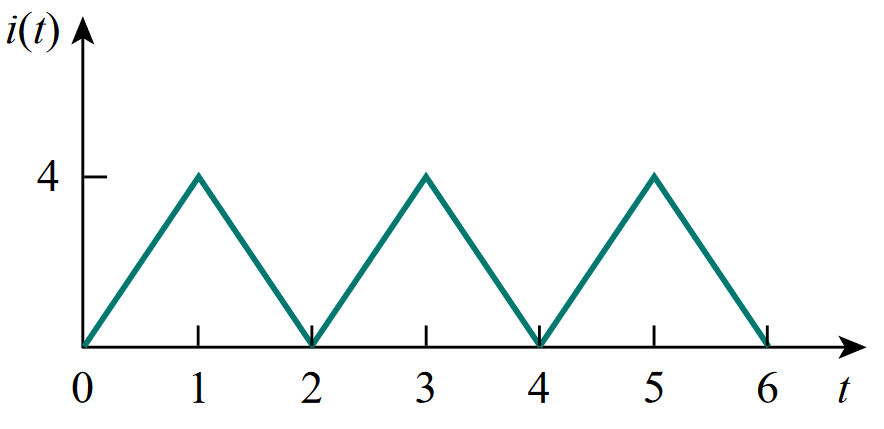
\includegraphics[width=0.4\textwidth]{Fig11.15_ElectricCircuit_SadikuPg446_3E}
			 \caption{}
             \label{fig:currentWaveform}
        \end{figure}
		


\begin{solution}

\end{solution}
%%%%%%%%%%%%%%%%%%%%%%%%%%%%%%%%%%%%%%%%%%%%%%%%%%%%%%%%%%			
\end{parts}

  	
%%%%%%%%%%%%%%%%%%%%%%%%%%%%%%%%%%%%%%%%%%%%%%%%%%%%%%%%%%
%%%%%%%%%%%%%%%%%%%%%%  Question#03  %%%%%%%%%%%%%%%%%%%%%
%%%%%%%%%%%%%%%%%%%%%%%%%%%%%%%%%%%%%%%%%%%%%%%%%%%%%%%%%%
\begin{comment}
  Put all the topics for this question.
\end{comment}
%%%%%%%%%%%%%%%%%%%%%%%%%%%%%%%%%%%%%%%%%%%%%%%%%%%%%%%%%%
\question 
\begin{parts}
%%%%%%%%%%%%%%%%%%%%%%%%%%%%%%%%%%%%%%%%%%%%%%%%%%%%%%%%%%	
\part[4]\color{red} If you want to place two figures side by side then use minipage environment. As for example: \color{black} Using nodal analysis, determine the potential across the \SI{4}{\Omega} resistor in Fig.~\ref{fig:ckt-nodal-analysis}
	

\begin{minipage}[t]{0.48\textwidth}
\begin{figure}[H]
\centering
\scalebox{0.7}{
\begin{tikzpicture}
	% Paths, nodes and wires:
	\draw (4, 4) to[american resistor, l_={$2~\Omega$}, label distance=0.02cm] (7, 4);
	\draw (7, 4) to[american resistor, l_={$2~\Omega$}, label distance=0.02cm] (10, 4);
	\draw (10, 4) to[american resistor, l={$4~\Omega$}, label distance=0.02cm] (10, 1);
	\draw (4, 4) to[american resistor, l={$2~\Omega$}, label distance=0.02cm] (4, 1);
	
	
	
	\draw (4, 4) to[american resistor, l={$5~\Omega$}, label distance=0.02cm] (7, 6);
	\draw (7, 6) to[american resistor, l={$5~\Omega$}, label distance=0.02cm] (10, 4);
	\draw (7, 1) to[american current source, l_={$3~A$}, label distance=0.02cm] (7, 4);
	\draw (4, 1) -- (10, 1);
	\draw node[ground] at (7, 1) {};
	\draw node[ground] at (7, 1) {};
	\draw node[ground] at (7, 1) {};
	\draw node[ground] at (7, 1) {};
\end{tikzpicture}
}

\caption{}
\label{fig:ckt-nodal-analysis}
\end{figure}
\vspace{0.5em}



\end{minipage}
\hfill
\begin{minipage}[t]{0.48\textwidth}
\begin{figure}[H]
\centering
\scalebox{0.7}{
\begin{tikzpicture}
	% Paths, nodes, and wires:
	\draw (5, 7) to[american resistor, l={$2~\Omega$}, label distance=0.02cm] (5, 4);
	\draw (5, 4) to[american resistor, l={$4~\Omega$}, label distance=0.02cm] (5, 1);
	\draw (8, 7) to[american resistor, l={$8~\Omega$}, label distance=0.02cm] (8, 4);
	\draw (8, 4) to[american controlled voltage source, l={$2~v_o$}, label distance=0.02cm] (8, 1);
	\draw (5, 4) to[american current source, l={$3~A$}, label distance=0.02cm] (8, 4);
	\draw (3, 7) to[american voltage source, l_={$12~V$}, label distance=0.02cm] (3, 1);
	\draw (3, 1) -- (8, 1);
	\draw (3, 7) -- (8, 7);


    \node at (4.5, 5.5) [align=center] {\textbf{+} \\[0.25cm] $v_o$ \\[0.25cm] \textbf{-}}; % Increased spacing above and below V_2


	% Loop current labels:
	\node at (4.0, 4.1) {$i_1$}; % Left loop
	\node at (6.7, 5.6) {$i_2$}; % Middle loop
	\node at (6.7, 2.6) {$i_3$}; % Right loop

	% Loop current direction arrows:
	\draw[->] (3.8, 4.5) arc[start angle=120, end angle=-150, radius=0.5]; % i1 loop arrow
	\draw[->] (6.5, 6) arc[start angle=120, end angle=-150, radius=0.5]; % i2 loop arrow
	\draw[->] (6.5, 3) arc[start angle=120, end angle=-150, radius=0.5]; % i3 loop arrow
\end{tikzpicture}
}

\caption{}
\label{fig:ckt-mesh-analysis}
\end{figure}

\vspace{0.5em}
\end{minipage}


\begin{solution}

\end{solution}
%%%%%%%%%%%%%%%%%%%%%%%%%%%%%%%%%%%%%%%%%%%%%%%%%%%%%%%%%%	
\part[4] Use mess analysis to find currents and voltage $v_o$ in the circuit of Fig.~\ref{fig:ckt-mesh-analysis}.
		
\begin{solution}

\end{solution}
%%%%%%%%%%%%%%%%%%%%%%%%%%%%%%%%%%%%%%%%%%%%%%%%%%%%%%%%%%
\part[2] \color{red}If a table is needed to insert, then you can use either tabular or tabulrx. In the table as shown in Table~\ref{table:someItems}, the data are given for a general purpose Silicon diode, draw the I-V characteristic curve. 

\color{black}
\begin{table}[H]
\centering
\caption{Your Table Title Here}
\label{table:someItems}
\begin{tabularx}{0.8\textwidth} { 
  | >{\raggedright\arraybackslash}X 
  | >{\centering\arraybackslash}X 
  | >{\raggedleft\arraybackslash}X | }
 \hline
 SL.no & Forward bias voltage (V) & Forward bias current(mA) \\
 \hline
  1 & 0 & 0 \\
 \hline
  2 & 0.2 & 0.0 \\
 \hline
  3 & 0.4 & 0.1 \\
 \hline
  4 & 0.5 & 0.5 \\
 \hline
  5 & 0.53 & 1.0 \\
 \hline
  6 & 0.6 & 8.2 \\
 \hline
  7 & 0.66 & 19.5 \\
 \hline
  8 & 0.7 & 53.5 \\
 \hline
  9 & 0.71 & 83.1 \\
 \hline
  10 & 0.73 & 112.7 \\
 \hline
 
\end{tabularx}
\end{table}



\begin{solution}

\end{solution}
%%%%%%%%%%%%%%%%%%%%%%%%%%%%%%%%%%%%%%%%%%%%%%%%%%%%%%%%%%
\end{parts}



%%%%%%%%%%%%%%%%%%%%%  	
%% The OR question
\begin{center}
\vspace{5mm}
\textbf{OR}
\vspace{5mm}
\end{center}	
%%%%%%%%%%%%%%%PART-A(Question#3OR
%%%%%%%%%%%%%%%%%%%%%%%%%%%%%%%%%%%%%%%%%%%%%%%%%%%%%%%%%%%%%%%%%%%%%%%%%%%%%%%%%%%%%%%%%%%%%%%%%%%%%	
%%%%%%%%%%%%%%%%%%%%%%%%%%%%%%%%%%%%%%%%%%%%%%%%%%%%%%%%%%%%%%%%%%%%%%%%%%%%%%%%%%%%
%%%%%%%%%%%%%%%%%% The OR question
\begin{parts}
%%%%%%%%%%%%%%%%%%%%%%%%%%%%%%%%%%%%%%%%%%%%%%%%%%%%%%%%%%%%%%%%%%%%	
\part [4]Find the Thevenin's equivalent circuit of Fig.~\ref{fig:ckt-thevenin-equivalent} to the left of the terminal.

\begin{figure}[H]
\centering
\begin{tikzpicture}
	% Paths, nodes, and wires:
	\draw (3, 3) to[american resistor, l={$5~\Omega$}, label distance=0.02cm] (6, 3);
	\draw (6, 3) to[american resistor, l={$3~\Omega$}, label distance=0.02cm] (9, 3);
	\draw (9, 3) to[american resistor, l={$4~\Omega$}, label distance=0.02cm] (9, -0);
	\draw (6, -0) to[american controlled current source, l_={$1.5I_x$}, label distance=0.02cm, mirror] (6, 3);
	\draw (3, 3) to[american voltage source, l_={$6~V$}, label distance=0.02cm] (3, -0);
	\draw (3, -0) -- (11, -0);
	\draw (9, 3) -- (11, 3);
	\draw node[ocirc] (N1) at (11, 3) {} node[anchor=west] at (N1.east){$a$};
	\draw node[ocirc] (N2) at (11, -0) {} node[anchor=west] at (N2.east){$b$};

	% Current label near the top left of 3Ω resistor:
	\node at (6.2, 3.6) {$I_x$};  % Label for the current
	\draw[->] (6.0, 3.3) -- (6.5, 3.3);  % Arrow indicating direction

\end{tikzpicture}
\caption{}
\label{fig:ckt-thevenin-equivalent}
\end{figure}

\begin{solution}

\end{solution}
%%%%%%%%%%%%%%%%%%%%%%%%%%%%%%%%%%%%%%%%%%%%%%%%%%%%%%%%%%%%%%%%%%%%
\part [4] Find the magnitude $R_L$ for the maximum power transfer in the circuit shown in Fig.~\ref{fig:ckt-max-power}. Also find out the maximum power. 

\begin{figure}[H]
\centering
\begin{tikzpicture}
	% Paths, nodes and wires:
	\draw (7.008, 4) to[american resistor, l_={$3~\Omega$}, label distance=0.02cm] (10.008, 4);
	\draw (1.008, 4) to[american resistor, l_={$5~\Omega$}, label distance=0.02cm] (1.008, 2.4);
	\draw (1.008, 2.4) to[battery1, l_={$10~V$}, label distance=0.02cm] (1.008, 1);
	\draw (4.008, 1) to[american current source, l={$6~A$}, label distance=0.02cm, mirror] (4.008, 4);
	\draw (10.008, 1) to[variable american resistor, l_={$R_L$}, label distance=0.02cm, mirror] (10.008, 4);
	\draw (1.008, 4) -- (7.008, 4);
	\draw (7.008, 1) to[american resistor, l={$4~\Omega$}, label distance=0.02cm] (10.008, 1);
	\draw (1.008, 1) -- (7.008, 1);
	\draw (7.008, 4) to[american resistor, l={$2~\Omega$}, label distance=0.02cm] (7.008, 1);
\end{tikzpicture}

\caption{}
\label{fig:ckt-max-power}
\end{figure}


\begin{solution}

\end{solution}
%%%%%%%%%%%%%%%%%%%%%%%%%%%%%%%%%%%%%%%%%%%%%%%%%%%%%%%%%%%%%%%%%%%%
\part[2] Write short notes on Real power and Reactive power. 


\begin{solution}

\end{solution}
%%%%%%%%%%%%%%%%%%%%%%%%%%%%%%%%%%%%%%%%%%%%%%%%%%%%%%%%%%%%%%%%%%%%
\end{parts}


	
%%%%%%%%%%%%%%%%%%%%%
%%%%%%%%%%%%%%%%%%%%%%%%%%%%%%%%%%%%%%%%%%%%%%%%%%%%%%%%%%%%%%%%%%%%%%%%%%%%%%%%%%%%%%%%%%%%%%%%%%%%%
%%%%%%%%%%%%%%%%%%%%%%%%%%%%%%%%%%%%%%%%%%%%%%%%%%%%%%%%%%%%%%%%%%%%%%%%%%%%%%%%%%%%%%%%%%%%%%%%%%%%%
%%%%%%%%%%%%%%%PART-B(Question#04--> 
%%%%%%%%%%%%%%%%%%%%%%%%%%%%%%%%%%%%%%%%%%%%%%%%%%%%%%%%%%%%%%%
%%%%%%%%%%%%%%%%%%%%%%%%%%%%%%%%%%%%%%%%%%%%%%%%%%%%%%%%%%%%%%%%%%%%%%%%%%%%%%%%	
\question 
\begin{parts} 
%%%%%%%%%%%%%%%%%%%%%%%%%%%%%%%%%%%%%%%%%%%%%%%%%%%%%%%%%%%%%%%%%	
\part[4]Determine $I_{BQ}$, $I_{CQ}$, $V_{CEQ}$, $V_B$, $V_C$ and $V_{BC}$ for the fixed-bias configuration shown in Fig.~\ref{fig:ckt-bjt-fixed-bias}. 
	
\begin{figure}[H]
\centering
\begin{tikzpicture}
	% Paths, nodes and wires:
	\draw node[npn] (N1) at (6, 4) {} node[anchor=west] at ([xshift=0.9cm]N1.east){$\beta = 50$};
	\draw (6, 7) to[american resistor, l^ ={\parbox{1cm}{\raggedright $R_C$ \\ $2.2~k\Omega$}}] (6, 4.77);
	\draw (5.16, 4) -- (2, 4);
	\draw (3, 7) to[american resistor, l^ ={\parbox{1cm}{\raggedright $R_B$ \\ $240~k\Omega$}}] (3, 4);
	\draw (3, 7) -- (6, 7);
	\draw node[circ] at (4.51, 7) {};
	\draw (4.5, 7) -| (4.5, 7.5);
	\draw node[ocirc] (N2) at (4.5, 7.5) {} node[anchor=south] at (N2.north){$V_{CC} = +12~V$};
	\draw (7.316, 4.77) to[curved capacitor, l={$C_2$}, label distance=0.02cm] (10.316, 4.8);
	\draw (2, 4) to[curved capacitor, l_={$C_1$}, label distance=0.02cm] (0, 4);
	\draw node[ground] at (6, 3.23) {};
	\draw node[ocirc] (N3) at (0, 4) {} node[anchor=east] at (N3.west){$ac~input$};
	\draw node[ocirc] (N4) at (10.316, 4.8) {} node[anchor=west] at (N4.east){$ac~output$};
	\draw (6, 4.77) -- (7.316, 4.77);
	\draw node[circ] at (3, 4) {};
	\draw node[circ, xscale=1.13, yscale=1.13] (N5) at (6, 4.77) {} node[anchor=north west] at ([xshift=-0.07cm, yshift=0.07cm]N5.east){$+$};

	% Label V_CE as an arc with arrows on both sides:
	\draw[<->] (6.3, 4.4) arc[start angle=90, end angle=-90, radius=0.4] node[midway, left] {$V_{CE}$};
	
	% Current I_B (Base Current) - Arrow towards base:
	\draw[->] (4, 4.2) -- (5.2, 4.2) node[midway, above] {$I_B$};

	% Current I_C (Collector Current) - Arrow down towards transistor:
	\draw[->] (5.7, 6.5) -- (5.7, 5.2) node[midway, left] {$I_C$};
	
	% Label capacitors with 10µF:
	\node at (1, 3) {10$\mu$F}; % Label for C1 (on the left capacitor)
	\node at (9.316, 4) {10$\mu$F}; % Label for C2 (on the right capacitor)
	
	

\end{tikzpicture}
\caption{}
\label{fig:ckt-bjt-fixed-bias}
\end{figure}



\begin{solution}


\end{solution}
%%%%%%%%%%%%%%%%%%%%%%%%%%%%%%%%%%%%%%%%%%%%%%%%%%%%%%%%%%%%%%%%%		
\part[2]Determine the saturation level for the network of Fig.~\ref{fig:ckt-bjt-fixed-bias}.

\begin{solution}


\end{solution}
%%%%%%%%%%%%%%%%%%%%%%%%%%%%%%%%%%%%%%%%%%%%%%%%%%%%%%%%%%%%%%%%%
\part[4]For the emitter bias network of Fig.~\ref{fig:ckt-bjt-emitter-bias} determine   $I_{B}$, $I_{C}$, $V_{CE}$, $V_C$, $V_E$ and $V_B$ for the fixed-bias configuration shown in 

\begin{figure}[H]
\centering
\begin{tikzpicture}
	% Paths, nodes and wires:
	\draw node[npn] (N1) at (6, 4) {} node[anchor=west] at ([xshift=0.88cm]N1.east){$\beta = 50$};
	\draw (6, 7) to[american resistor, l={$2~k\Omega$}, label distance=0.02cm] (6, 4.77);
	\draw (5.16, 4) -- (2, 4);
	\draw (3, 7) to[american resistor, l_={$430~k\Omega$}, label distance=0.02cm] (3, 4);
	\draw (3, 7) -- (6, 7);
	\draw node[circ] at (4.51, 7) {};
	\draw (4.5, 7) -| (4.5, 7.5);
	\draw node[ocirc] (N2) at (4.5, 7.5) {} node[anchor=south] at (N2.north){$ +20~V$};
	\draw (7.316, 4.77) to[curved capacitor, l={$10~\mu F$}, label distance=0.02cm] (10.316, 4.8);
	\draw (2, 4) to[curved capacitor, l_={$10~\mu F$}, label distance=0.02cm] (0, 4);
	\draw node[ocirc] (N3) at (0, 4) {} node[anchor=east] at (N3.west){$v_i$};
	\draw node[ocirc] (N4) at (10.316, 4.8) {} node[anchor=west] at (N4.east){$v_o$};
	\draw (6, 4.77) -- (7.316, 4.77);
	\draw node[circ] at (3, 4) {};
	\draw node[circ, xscale=1.13, yscale=1.13] at (6, 4.77) {};
	\draw (6, 3.23) to[american resistor, l={$1~k\Omega$}, label distance=0.02cm] (6, 1);
	\draw (8, 2.5) to[capacitor, l={$40~\mu F$}, label distance=0.02cm] (8, 1);
	\draw (6, 3.23) -| (8, 2.5);
	\draw node[tlground] at (6, 1) {};
	\draw node[tlground] at (6, 1) {};
	\draw node[tlground] at (8, 1) {};
	\draw node[tlground] at (8, 1) {};
	\draw node[circ] at (6, 3.23) {};
\end{tikzpicture}

\caption{}
\label{fig:ckt-bjt-emitter-bias}

\end{figure}


\begin{solution}


\end{solution}
%%%%%%%%%%%%%%%%%%%%%%%%%%%%%%%%%%%%%%%%%%%%%%%%%%%%%%%%%%%%%%%%%	
\end{parts}
  	

%%%%%%%%%%%%%%%%%%%%%%%%%%%%%%%%%%%%%%%%%%%%%%%%%%%%%%%%%%
%%%%%%%%%%%%%%%%%%%%%%  Question#05  %%%%%%%%%%%%%%%%%%%%%
%%%%%%%%%%%%%%%%%%%%%%%%%%%%%%%%%%%%%%%%%%%%%%%%%%%%%%%%%%
\begin{comment}
  Put all the topics for this question.
\end{comment}
%%%%%%%%%%%%%%%%%%%%%%%%%%%%%%%%%%%%%%%%%%%%%%%%%%%%%%%%%%
		
\question [12] With Lorentz Oscillator Model, find an expression for dielectric displacement field, $D$. 

\begin{solution}

\end{solution}
%%%%%%%%%%%%%%%%%%%%%%%%%%%%%%%%%%%%%%%%%%%%%%%%%%%%%%%%%%		

  	


%%%%%%%%%%%%%%%%%%%%%%%%%%%%%%%%%%%%%%%%%%%%%%%%%%%%%%%%%%%%%%%%%%%%%%%%%%%%%%%%%%%%%%%%%%%%%%%%%%%%%
%%%%%%%%%%%%%%%PART-B(Question#06--%%%%%%%%%%%%%%%%%%%%%%%%%%%%%%%%%%%%%%%%%%%%%%%%%%%%%%%%%%%%%%%%%%
\question 
\begin{parts}
%%%%%%%%%%%%%%%%%%%%%%%%%%%%%%%%%%%%%%%%%%%%%%%%%%%%%%%%%%%%%%%%%%%%%	
\part[4]Simplify the Boolean function $F(w, x, y, z) = \sum (1, 3, 7, 11, 15)$. Which has don't-care condition: $d(w, x, y, z) = \sum(0, 2, 5)$. 

\begin{solution}

\end{solution}
%%%%%%%%%%%%%%%%%%%%%%%%%%%%%%%%%%%%%%%%%%%%%%%%%%%%%%%%%%%%%%%%%%%%%
\part[4]Simplify $F(A, B, C, D) = \sum(0, 1, 2, 5, 8, 9, 10)$ in product of sums.


\begin{solution}

\end{solution}
%%%%%%%%%%%%%%%%%%%%%%%%%%%%%%%%%%%%%%%%%%%%%%%%%%%%%%%%%%%%%%%%%%%%%
\part[2]Define Minterms and Maxterms and briefly explain De Morgan's law.


\begin{solution}

\end{solution}
%%%%%%%%%%%%%%%%%%%%%%%%%%%%%%%%%%%%%%%%%%%%%%%%%%%%%%%%%%%%%%%%%%%%%		
\end{parts}
			
  	

%%%%%%%%%%%%%%%%%%%%%
\begin{center}
\vspace{5mm}
\textbf{OR}
\vspace{5mm}
\end{center}	
%%%%%%%%%%%%%%%%%% The OR question
	
\begin{parts}
%%%%%%%%%%%%%%%%%%%%%%%%%%%%%%%%%%%%%%%%%%%%%%%%%%%%%%%%%%%%%%%%%%%%%%		
\part[4]Simplify the Boolean function $F(w, x, y, z) = \sum(0, 1, 2, 4, 5, 6, 8,9, 12, 13, 14)$. 


\begin{solution}
	
\end{solution}	
%%%%%%%%%%%%%%%%%%%%%%%%%%%%%%%%%%%%%%%%%%%%%%%%%%%%%%%%%%%%%%%%%%%%%%		
\part[4] Suppose you have 3 friends. Design an alarm which will ring when more than one friend come. 

\begin{solution}
	
\end{solution}		
%%%%%%%%%%%%%%%%%%%%%%%%%%%%%%%%%%%%%%%%%%%%%%%%%%%%%%%%%%%%%%%%%%%%%%		
\part[2\half]Draw the symbol and truth table of EX-OR gate \& EX-NOR gate.

\begin{solution}
	
\end{solution}		
%%%%%%%%%%%%%%%%%%%%%%%%%%%%%%%%%%%%%%%%%%%%%%%%%%%%%%%%%%%%%%%%%%%%%%
\end{parts}

	
%%%%%%%%%%%%%%%%%%%%%
%%%%%%%%%%%%%%%%%%%%%%%%%%%%%%%%%%%%%%%%%%%%%%%%%%%%%%%%%%%%%%%%%%%%%%%%%%%%%%%%%%%%%%%%%%%%%%%%%%%%			
%%%%%%%%%%%%%%%%%%%%%%%%%%%%%%%%%%%%%%%%%%%%%%%%%%%%%%%%%%%%%%%%%%%%%%%%%%%%%%%%%%%%%%%%%%%%%%%%%%%%
\end{questions}
%%%%%%%%%%%%%%%%%%%%%%%%%%%%%%%%%%%%%%%%%%%%%%%%%%%%%%%%%%%%%%%%%%%%%%%%%%%%%%%%%%%%%%%%%%%%%%%
%% If you want to provide some formuls
\vfill
%%%% The list of given formulas
\begin{center}
\textbf{List of the relevant equations:}

\[
\begin{aligned}
\begin{bmatrix}
A_r \\
A_{\theta} \\
A_{\phi}
\end{bmatrix}
&=
\begin{bmatrix}
\sin\theta \cos\phi & \sin\theta \sin\phi & \cos\theta \\
\cos\theta \cos\phi & \cos\theta \sin\phi & -\sin\theta \\
-\sin\phi & \cos\phi & 0
\end{bmatrix}
\begin{bmatrix}
A_x \\
A_y \\
A_z
\end{bmatrix} \\[1.5em]
\nabla \times \mathbf{A}
&=
\frac{1}{r \sin\theta}
\begin{vmatrix}
\hat{r} & r \hat{\theta} & r \sin\theta \hat{\phi} \\
\dfrac{\partial}{\partial r} & \dfrac{\partial}{\partial \theta} & \dfrac{\partial}{\partial \phi} \\
A_r & r A_\theta & r \sin\theta A_\phi
\end{vmatrix} \\[1.2em]
&=
\frac{1}{r \sin\theta}
\Bigg[
\hat{r} \left(
\frac{\partial}{\partial \theta}\!\big(\sin\theta A_\phi\big) -
\frac{\partial A_\theta}{\partial \phi}
\right)
+ \hat{\theta} \left(
\frac{1}{\sin\theta}\frac{\partial A_r}{\partial \phi} -
\frac{\partial}{\partial r}(r A_\phi)
\right) \\
&\qquad\qquad
+ \hat{\phi} \left(
\frac{\partial}{\partial r}(r A_\theta) -
\frac{\partial A_r}{\partial \theta}
\right)
\Bigg] \\[1.5em]
\begin{bmatrix}
a_x \\
a_y \\
a_z
\end{bmatrix}
&=
\begin{bmatrix}
\sin\theta \cos\phi & \cos\theta \cos\phi & -\sin\phi \\
\sin\theta \sin\phi & \cos\theta \sin\phi & \cos\phi \\
\cos\theta           & -\sin\theta          & 0
\end{bmatrix}
\begin{bmatrix}
a_r \\
a_{\theta} \\
a_{\phi}
\end{bmatrix}.
\end{aligned}
\]



\end{center}




\ifprintanswers
	%Stuff to appear only when answers \textbf{are} being printed.
\else
	%Stuff to appear only when answers \textbf{are not} being printed.
\fi


\end{document}
